\documentclass[12pt]{article}

\setlength\parindent{0pt}
\newcommand{\myt}[1]{\textbf{\underline{#1}}}

\usepackage{mathtools}
\usepackage{amssymb}
\usepackage{tikz,ifthen,amsmath,amssymb,fancyhdr,comment,lastpage}

\title{\vspace{-15ex}CS 240 Module 3\vspace{-1ex}}
\date{May 4th, 2015}
\author{Graham Cooper}

\begin{document}
	\maketitle
	
	\section*{Selection}
	Given an array A$[a...n-1]$ and $0 \leq k \leq n-1$ return the kth largest element in A.\\
	
	\subsection*{1) Selection-sort Idea:}
	Scan A k times, deleting max each time.\\
	Cost: $\Theta(kn)$\\
	\subsection{2)}
	Sort A, return A[n-k]\\
	Cost: $\Theta(nlogn)$\\
	
	\subsection*{3)}
	Scan the array once, and keep k largest seen so far in the min-heap.\\
	Cost: $\Theta(nlogk)$\\
	Eg: [6,5,3,8,7,4], k =3\\
	We put in 6, 5 then 3 into the min heap. After we look at the rest of the elements and keep the min heap the size of k and add new elements if an element in the array is larger than the root of the min-heap. Continue through the array and at the end pick the root of the min heap.
	
	\subsection*{4)}
	Heapify(A) then call deleteMax k times.\\
	Cost: $\Theta(n + klogn)$ For median selection (k = n/2) then it is the same as sorting so $\Theta(n)$\\
	
	
	
	\section*{Partition Algorithm}
	Given an array A[0...n-1] and $0 \leq k \leq n-1$, find the element at position k of the sorted A.\\
	
	\myt{Observation:}\\
	A = $[\overset{0}{7}, \overset{1}{3}, \overset{2}{2}, \overset{3}{4}, \overset{4}{6}, \overset{5}{1}]$\\
	Sorted(A) = [1, 2, 3, 4, 6, 7]\\
	What is the position of A[3](4) in the sorted A. the answer is the number of elements $<$ A[3] in A[0..2] and A[4,5]\\
	
	\myt{Idea:} choose one element (pivot) and partition the data into: (items $<$ pivot), pivot, (items $>$ pivot). If position(pivot) == k, done, otherwise, continue either on the left or on the right, depending on the position of the pivot.\\
	
	WHAT WE WANT TO DO:\\
	
	Implicit A = $[\overset{0}{9}, \overset{1}{4}, \overset{2}{5}, \overset{3}{8}, \overset{4}{6}, \overset{5}{3}, \overset{6}{2}]$\\
	
	Lets pick A[2] as the pivot, swap A[2] and A[0]\\
	A = [5,4,9,8,6,3,2]\\
	
	\myt{Idea:} Find the outermost wrongly positioned pair and swap.\\
	
	advance i, backup j.\\
	A = [5, 4, 9, 8, 6, 3, 2]\\
	$i < j$ so we should swap i\\
	A = [5, 4, 2, 8, 6, 3, 9]\\
	Advance i, backup j\\
	A = [5, 4, 2, 8 ,6 ,3, 9]\\
	$i < j$ swap i\\
	A = [5, 4, 2, 3, 6 ,8 ,9]\\
	advance i, backup j\\
	A = [5, 4, 2, 3, 6, 8 ,9]\\
	$j < i$ stop, swap, A[0] wiht A[j]\\
	A = [3, 4, 2, 5, 6, 8, 9]\\
	Return 3.\\
	
	\subsection*{Quick Select(A,K)}
	P = choosePivot(A)\\
	i = partition(P)\\
	if i = k\\
	return A[i]\\
	if i $>$ k:\\
	return QuickSelect(A[0...i-1], k)\\
	if i $<$ k:\\
	return QuickSelect(A[i+1...n-1], k-i-1)\\
	
	\subsubsection{Cost of Quick Select}
	Let T(n) e cost of QuickSelect\\
	T(n) = $\Theta(n) + $\\
	$\Theta(1)$, if n = k\\
	T(i) if $i > k$\\
	T(n-i-1), if $i < k$\\
	
	\myt{Best Case:} T(n) = $\Theta(n)$ if i = k\\
	(first chosen pivot if the element at position k, no recursive calls)\\
	
	\myt{Worst Case:} i = 0 or i = n-1\\
	Recursive call has size n - 1\\
	(if we pick the first element as the pivot, then an array sorted in ascending or descending order will give the worst case runtime.)\\
	
	T(n) = \\
	d if n = 1\\
	T(n-1) + cn if n $\geq$ 2\\
	T(n) = cn + c(n-1) + c(n-2) + ... + c(2) + d\\
	= $c)\frac{n(n+1)}{2} - c + d \in \Theta(n^2)$\\
	
	\myt{What if hte partition is balanced}\\
	A[p] is always close to median\\
	T(n) = \\
	T($\frac{n}{2}) + cn$ if n $\geq$ 2\\
	d if n = 1\\
	
	Assume n is a power of 2: $2^x$\\
	$T(2^x) = c \cdot 2^x + c \cdot 2^{x-1} + ... + c \cdot 2 + d$\\
	$ = c(2^{x+1} - 2) + d$\\
	$ = 2c(n-1) + d \in \Theta(n)$\\
	
	\myt{Average-Case analysis}: Average cost over all inputs of size n as function of n.\\
	\underline{Observation}: behaviour of QuickSelect depends on relative ordering, and not on actual values. [1,3,5,7] will yeild the same worst case behaviour as [4,5,6,7].\\
	
	Assume all keys are unique, $x_1, x_2,...x_n$ then there are n! possible orderings on these keys. and each ordering is equally likely\\
	
	After we pick the pivot, what iwll the split look like?\\
	\begin{tabular}{c | c}
		L(num of items) & R(num of items) \\ \hline
		0 & n-1 \\
		1 & n-2 \\
		... & ...\\
		k - 1 & n - k\\
		k & n - k - 1 \\
		k + 1 & n - k - 2\\
		... & ... \\
		n - 1 & 0 \\
	\end{tabular} 
	
	For each choce of pivot (n possible pivots) there are (n-1)! permutations of non-pivot elements, each of the splits is equally likely\\
	
	After Partiction:\\
	A = [0...x...]\\
	Define T(n,k) an average cost for selecting kth item from a size n array.\\
	
	$$T(n,k) = cn + \frac{1}{n}T(n-1, k-1)x + \frac{1}{n}(n-2, k-2) + ... \frac{1}{n}T(n-1, k)$$
	$$cn + \frac{1}{n}(\sum_{i=1}^{k-1}T(n-i-1, k=i=1) + \sum_{i=k+1}^{n-1}T(o,k))$$
	Put in summation notation.\\
	
	Define T(n) = max T(n,k) $0 \leq k \leq n-1$\\
	
	\myt{Observation}:
	$[\_\_\overset{n/2}{|}\_\_X\_\_\overset{3n/4}{|}\_\_]$
	pivot ends up in between the two divisions. At least 1/2 of all the n1 problem instances will have the pivot at position n/4 $\leq$ i $<$ 3n/4\\
	
	For these instances, recursive call has length at most floor($\frac{3n}{4}$), no matter what k is.\\
	
	$T(n) \leq $:\\
	if $n \geq 2$\\
	cn + 1.2(T(n) + T(floor($\frac{3n}{4}))$\\
	if $n = 1$\\
	d\\
	
	$$T(n) \leq 2cn + T(floor(\frac{3n}{4})) \leq 2cn + T(\frac{3n}{4})$$
	$$\leq 2cn + 2c(\frac{3n}{4}) + 2c(\frac{9n}{16}) + ... + d$$
	$$= d + 2cn \sum_{i=0}^{\infty}(\frac{3}{4})^i \leq d 2cn \times 4 \in O(n)$$
	$T(n) \in \Omega(n)$ Since we have to parition at least once $T(n) \in \Omega(n)$\\
	
	Worst case runtime is $\Theta(n^2)$\\
	
	Your enemy could make your algorith mrun slowly by a "Bad" order input.\\
	Another approach: Randomized quickSelect.\\
	- Pick Pivot at random\\
	- No ordering of the input on its own is guaranteed ot be bad
	
	\myt{The expected runtime:} with prob at least 1/2 the pivot will randomly fall between roof(n/4) and floor(3n/4), so the analysis is the same as for the average case: $\Theta(n)$\\
	
	\subsubsection*{Finding a Pivot}
	\myt{Idea:} generate a good pivot deterministically (median of medians), assume all keys are distinct\\
	\begin{enumerate}
		\item Divide the array into x = n/5 groups of 5 elements each
		\item find the median of each group
		\item Recursively select the median among the medians of these groups
		\item Partition with the median found in Step 3 as a pivot
		\item Recurse in appropriate part of the array, $k \neq i$
	\end{enumerate}
	Step 1 + Step 2: $\Theta(n)$\\
	Step 3: $T(\frac{n}{5})$\\
	Step 4: $\Theta(n)$\\
	Step 5: T(?)\\
	
	The recurrence relation is T(n) $\leq$
	
	\subsection*{QuickSort A[0...n-1]}
	\begin{verbatim}
	if n <= 1 return
	p = choose_pivot(A)
	i = partition(A,p)
	QuickSort(A[0...i-1])
	QuickSort(A[i+1 ... n-1])
	\end{verbatim}
	
	\subsubsection*{Worst-Case:}
	Pivot ends up at one end or the other after positioning.\\
	T(n) = cn + T(n-1) $\in \Theta(n^2)$\\
	
	\subsubsection*{Best Case}
	T(n) = T(floor($\frac{n-1}{2}$)) + T(roof($\frac{n-1}{2}$) + cn $<$ 2T(n/2) + cn $\Theta$(nlogn)\\
	
	What if our partition always splits n/10 and 9n/10\\
	T(n) = \\
	if $n \leq 1$\\
	d\\
	if $n > 1$\\
	T(n/10) + T(9n/10) + cn\\
	
	RECURSION TREE NO ON THIS PAGE\\
	
	$$T(n) \leq cn \cdot log_{\frac{10}{9}}(n) + cn \in \Theta(nlogn)$$
	
	\subsubsection*{Average Case}
	$[\_\_\overset{n/2}{|}\_\_X\_\_\overset{3n/4}{|}\_\_]$\\
	
	i, n-i-1 average sizes of two subproblems, taking average cost over all n possibilitys of i.\\
	
	$$T(n) = cn + \frac{1}{n}\sum_{i=0}^{n-1}(T(i) + T(n-i-1))$$
	$$ = cn + \frac{1}{n} \cdot 2 \sum_{i=0}{n-1}T(i), n \geq 2$$
	
	NEW STUFF
	
	$$nT(n) = cn^2 + 2(T(0) + T(1) + ... + T(n-1))$$
	$$(n-1)T(n-1) = c(n-1)^2 + 2(T(0) + T(1) + ... + T(n-2))$$
	$$nT(n) - (n-1)T(n-1) = 2cn - c + 2T(n-1)$$
	$$nT(n) = (n+1)T(n-1) + 2cn - c$$
	$$\frac{T(n)}{n+1} = \frac{T(n-1)}{n} + \frac{2cn - c}{n(n+1)}$$
	$$ < \frac{T(n-1)}{n} + \frac{2c}{n+1}$$
	
	$$\frac{T(n-1)}{n} \leq \frac{T(n-2)}{n-1} + \frac{2c}{n}$$
	$$\frac{T(n-2)}{n-1} \leq \frac{T(n-3)}{n-2} + \frac{2c}{n-1}$$
	$$\frac{T(n)}{n+1} \leq \frac{T(n-1)}{n} + \frac{2c}{n+1} \leq \frac{T(n-2)}{n-1} + \frac{2c}{n} + \frac{2c}{n+1}$$
	$$\frac{T(n-3)}{n-2} + \frac{2c}{n-1} + \frac{2c}{n} + \frac{2c}{n + 1} ...$$
	$$\frac{T(1)}{2} + \frac{2c}{3} + \frac{2c}{4} + .. + \frac{2c}{n+1} = $$
	$$= \frac{d}{2} + 2c\sum_{i=3}^{n+1}\frac{1}{i} = \frac{d}{2} + 2c(H_{n+1} - H_{2})$$
	$$\in O(logn)$$
	$$\frac{T(n)}{n+1} \in O(logn) \ implies T(n) \in O(logn)$$
	
	\section*{QuickSort}
	
	\subsection*{Avg. Case Analysis of Quick Sort}
	Assume pivot is at index i\\
	$$T(n) = cn + T(i) + T(n-i - 1)$$
	How many sequences do we have? $->$ n!\\\
	$$T(n) = \frac{1}{n!}(\sum_{i=1}^{n}(cn + T(i) + T(n-i-1)) \cdot (n-1)!$$
	$$= cn + frac{1}{n}(\sum_{i=1}^{n}T(i) + T(n-i-1)$$
	$$= cn + \frac{1}{n}\sum_{i=1}^{n}T(i) + \frac{1}{n}\sum_{j=1}^{n}T(j)$$
	$$T(n) = cn + \frac{2}{n}\frac{2}{n}\sum_{i=1}^{n}T(i)$$
	$$nT(n) = cn^2 + 2 \sum_{i=1}^{n}T(i)$$
	$$(n-1)T(n-1) = c(n-1)^2 + 2\sum_{i=0}^{n-2}T(i)$$
	$$nT(n) - (n-1)T(n-1) = 2cn - c + 2T(n-1)$$
	$$nT(n) = 2cn - c + (n+1)T(n-1)$$
	$$\frac{T(n)}{n+1} = \frac{T(n-1)}{n} + \frac{2c}{n+1}$$
	$$\frac{T(n)}{n+1} \leq \frac{T(n-2)}{n-1} + \frac{2c}{n+1} = \frac{2c}{n}$$
	$$\frac{T(n)}{n+1} = \frac{T(n-3)}{n-1} + \frac{2c}{n+1} + \frac{2c}{n} + \frac{2c}{n-1}$$
	$$...$$
	$$...$$
	$$\frac{T(n)}{n+1} \leq \frac{2c}{n+1} + \frac{2c}{n} + \frac{2c}{n-1} + ... \frac{2c}{2} + 2c$$
	$$\frac{T(n)}{n+1} \leq 2cln(n)$$
	$$T(n) \leq (n+1)(n(n) 2c) \in \Theta(nlogn)$$
	
	\subsection*{More Notes on Quicksort}
	\begin{verbatim}
	Q-sort(A,L,R){
		if(n < 2) break
		
		piv <- partition(A,L,R)
		Q-sort(A,L,piv=1)
		Q-sort(A,piv+1, R)
	}
	\end{verbatim}
	M(n) = memory\\
	$$M(n) = 2M(\frac{n}{2}) + C$$
	Two recursive calls each require its own stream on the stack space\\
	$$M(n) \in \Theta(n)$$
	
	\begin{verbatim}
	Tail_Rec_Q-sort(A,L,R){
		if(R-L) < 2 Break;
		piv <- partition(A,L,R)
		if(a < (R-L)/2){
			Tail_Rec_Q-sort(A,L,piv-1)
			L=Piv+1
		} else {
			Tail_Rec_Q-sort(A, piv+1, R)
			R=Piv-1
		}
	}
	\end{verbatim}
	
	$$M(n) \leq M(\frac{n}{2} + c) \in \Theta(logn)$$
	
	\section*{Comparison Based Model}
	Sort objects (POTATOES) by mutual comparison\\
	
	Assume $P_1, P_2, P_3 ... P_n$\\
	Assume the cost fora comparison is 1,everything else is free.\\
	
	Each comparison divides the number of possibilities by 2.\\
	Starts with n! permuations, then $\frac{n!}{2} ...$\\
	- Binary tree\\
	-- Each node is a comparison\\
	-- each leaf is a permutation\\
	- A binary tree with n! leaves\\
	
	A binary tree with n! leaves\\
	- Even if it is full, the height is at least $\Omega(logn)$\\
	- ot am ne for wordst (eg, O(n!))\\
	
	\section*{Counting Sort}
	n integers all smaller than m\\
	size m\\
	C:\\
	\begin{tabular}{| c | c | c | c | c | c |}
		\hline
		0 & 0 & 0 & 0 & 0 & 0 \\ \hline	
	\end{tabular}
	\begin{tabular}{| c | c | c | c | c | c |}
		\hline
		1 & 2 & 3 & 1 & 0 & 1 \\ \hline	
	\end{tabular}
	
	\begin{enumerate}
		\item count the number of occurances in array c
		\item In new array L find left boundaries L[i] = L[i-1] + C[i-1]
	\end{enumerate}
	
	L:
	\begin{tabular}{| c | c | c | c | c | c |}
		\hline
		0 & 1 & 3 & 6 & 8 & 8 \\ \hline	
	\end{tabular}
	
	1. Count how many times each number appears\\
	
	Eg. \\
	A=
	\begin{tabular}{| c | c | c | c | c | c | c | c | c | c|}
		\hline
		2 & 3 & 1 & 2 & 0 & 5 & 3 & 2 & 1 & 5 \\ \hline
		L & I & F & E & I & S & G & O & O & D \\ \hline
	\end{tabular}
	\\
	C= 
	\begin{tabular}{| c | c | c | c | c | c |}
		\hline
		0 & 1 & 2 & 3 & 4 & 5  \\ \hline
		1 & 2 & 3 & 2 & 0 & 2 \\ \hline
	\end{tabular}
	
	2. Create L $\rightarrow$ L[i] $\rightarrow$ number of keys smaller than i\\
	L[i] = L[i-1] + c[i-1] $\rightarrow$ Left Boundary\\
	L=
	\begin{tabular}{| c | c | c | c | c | c |}
		\hline
		0 & 1 & 2 & 3 & 4 & 5  \\ \hline
		0 & 1 & 3 & 6 & 8 & 8 \\ \hline
	\end{tabular}\\
	\begin{tabular}{| c | c | c | c | c | c |}
		\hline
		0 & 1 & 2 & 3 & 4 & 5  \\ \hline
		1 & 2 & 5 & 7 & 8 & 8 \\ \hline
	\end{tabular}\\
	\begin{tabular}{| c | c | c | c | c | c |}
		\hline
		0 & 1 & 2 & 3 & 4 & 5  \\ \hline
		1 & 3 & 6 & 8 & 8 & 10 \\ \hline
	\end{tabular}
	
	B= 
	\begin{tabular}{| c | c | c | c | c | c | c | c | c | c |}
		\hline
		0 & 1 & 2 & 3 & 4 & 5 & 6 & 7 & 8 & 9 \\ \hline
		0 & 1 & 1 & 2 & 2 & 2 & 3 & 3 & 5 & 5  \\ \hline
	\end{tabular}
	
	\section*{Radix Sort}
	A set of n positive integers that have m digits in bas R.\\
	
	\begin{tabular}{c | c | c | c | c | c | c | c }
		m=3 & 420 & 318 & 418 & 975 & 317 & 119 & 019 \\
		r = 10 & 019 & 119 & 318 & 317 & 420 & 418 & 973 \\
		n = 7 & 019 & 119 & 317 & 318 & 418 & 420 & 973 \\
	\end{tabular}\\
	
	Most Significant Digits\\
	\begin{enumerate}
		\item Partition by most significant dgiit using counting sort
		\item Recurse on each "bin" including numbers with the same MSD
	\end{enumerate}
	
	Lease Significant Digits\\
	\begin{enumerate}
		\item For d from LSD to MSD
		\item Sort by d'th digit $\rightarrow$ use d'th aas the key for counting sort
	\end{enumerate}
	\begin{tabular}{c | c | c | c | c | c | c | c }
		m=3    & 420 & 318 & 418 & 975 & 317 & 199 & 019 \\
		r = 10 & 420 & 973 & 317 & 318 & 418 & 199 & 019 \\
		n = 7  & 317 & 318 & 418 & 019 & 420 & 973 & 199 \\
		       & 019 & 119 & 317 & 318 & 418 & 420 & 973 \\
	\end{tabular}\\
	
	LSD for n numbers $\leq$ n of R = 10, m = log$_{10}^n \in \Theta(logn)$\\
	m(n + R) $\in \Theta(nlogn)$\\
	
	\section*{Binary Search Trees (review)}
	
	Given n (positive) integers of value at most $n^5$ how can we sort in O(n)?\\
	
	Radix sort $->$ Base R = n $->$ m(n+R) $\in \Theta(n)$\\
	
	\subsection*{Height of a BST}
	
	
	\subsubsection*{Worst Case}
	$h \in \Theta(n)$\\
	
	\begin{center}\begin{tikzpicture}[
		level distance=45 pt,
		every node/.style={circle,draw},
		level 1/.style={sibling distance=200 pt},
		level 2/.style={sibling distance=100 pt},
		level 3/.style={sibling distance=60 pt}
		]
		\node {10}
		child {node {9}
			child {node {8}
				child {node {7}
					child {node {6}
						child {node {5}
							child {node {4}
							child [missing]
						}
						child [missing]
					}
					child [missing]
				}
				child [missing]
			}
			child [missing]
		}
		child[missing]
	};
	\end{tikzpicture}\end{center}
	
	\subsubsection*{Best Case}
	
	%% FIX THIS
	\begin{center}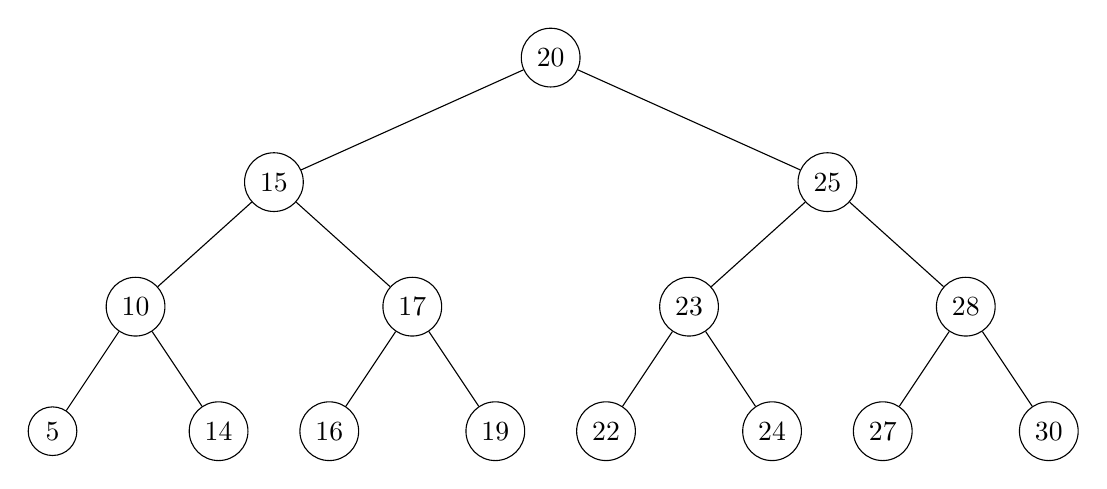
\begin{tikzpicture}[
		level distance=45 pt,
		every node/.style={circle,draw},
		level 1/.style={sibling distance=200 pt},
		level 2/.style={sibling distance=100 pt},
		level 3/.style={sibling distance=60 pt}
		]
		\node {20}
			child {node {15}
				child {node {10}
					child {node {5}}
				child {node {14}}
			}
			child {node {17}
				child{node {16}}
				child{node {19}}
			}
		}
			child{node {25}
				child{node {23}
					child {node {22}}
					child {node {24}}
				}
				child{node {28}
					child {node {27}}
					child {node {30}}
				}
			}
		;
	\end{tikzpicture}\end{center}
	
	\subsubsection*{Average Case}
	$$H(n) = 1 + \frac{1}{n}\sum_{i = 0}^{n-1}max\{H(i), H(n-i-1)\}$$
	$$= 1 + \frac{1}{n}(\sum_{i=1}^{floor(frac{n}{2} - 1)}H(n-i-1) + \sum_{i=floor(\frac{n}{2}}^{n-1}H(i))$$
	$$ = 1 + \frac{1}{n}(\sum_{j=n-floor(\frac{n}{2})}^{n-1} H(j) + \sum_{i = floor(\frac{n}{2})}^{n-1} H(i)$$
	$$ H(n) \leq 1 + \frac{2}{n}\sum_{i = floor(\frac{n}{2})}^{n-1} H(i)$$
	$$= 1 + \frac{2}{n}(\sum_{i = floor(\frac{n}{2})}^{\frac{3n}{4}}H(i) + \sum_{i = \frac{3n}{4} + 1}^{n-1} H(i))$$
	$$H(n) \leq 1 + \frac{2}{n} \times \frac{n}{4} \times H(\frac{3n}{4}) + \frac{2}{n} \times \frac{n}{4} \times H(n)$$
	$$H(n) \leq 1 + \frac{1}{2}H(\frac{3n}{4}) + \frac{1}{2}H(n)$$
	$$H(n) \leq 2 + H(\frac{3n}{4})$$
	$$H(n) \leq 2 + 2 + H(\frac{9n}{16})$$
	$$\leq 2 + 2 + .... + 2 = 2 \times log_{\frac{4}{3}}^n \in O(logn)$$
	
	\subsection*{Balanced BSTs}
	\begin{itemize}
		\item The goal is to have height $\Theta(logn)$ ALWAYS
		\item For that, we consider balance-factor$->$BF
		\item BF(x) = height(x $->$ right) - height(x $->$ left)
		\item height(null) = -1
	\end{itemize}
	
	We call a node x
	\begin{itemize}
		\item left heavy if bf(x) $<$ 0
		\item right heavy if bf(x) $>$ 0
		\item balanced if BF = 0
	\end{itemize}
	
	\subsection*{AVL Tree}
	An AVL tree is a BST such that the BF of all nodes is either -1, 0 and 1
	
\end{document}

























